% E1-E2 methodology + results. Also the source for report chapter 5 (part A). Owner: Saket.
\paragraph{Data and tokenizers.}
We use the 1{,}012 sentences of the FLORES-200 devtest split \citep{nllb2022} in English and \nLangs{}
Indian languages (Hindi, Marathi, Bengali, Assamese, Gujarati, Punjabi, Odia, Urdu, Tamil, Telugu,
Kannada, Malayalam), NFC-normalised. Because the sentences are translations of each other, token
counts compare the cost of the \emph{same content}. We audit \texttt{cl100k\_base} and
\texttt{o200k\_base} (tiktoken) and the Hugging Face tokenizers of Llama~3, Qwen2.5, Gemma~2, XLM-R and
Sarvam-1, always without special tokens. \todo{Llama 3 pending licence approval}

\paragraph{Metrics.}
For tokenizer $\tau$ and language $\ell$, summing over all sentences $c$:
\begin{equation*}
T_\tau(\ell)=\frac{\sum_c|\tau(x_\ell(c))|}{\sum_c|\tau(x_{\ell_0}(c))|},\qquad
F_\tau(\ell)=\frac{\sum_c|\tau(x_\ell(c))|}{\sum_c \mathrm{words}(x_\ell(c))},
\end{equation*}
where words are whitespace-separated. The \emph{tax} $T$ is a ratio of total tokens for the same content,
so English is exactly 1. The \emph{single-byte rate} $\sigma_\tau(\ell)$ is the share of tokens whose bytes
are not a complete UTF-8 character, i.e.\ merges that failed inside a character.

We report $T$ rather than the fertility ratio $F_\tau(\ell)/F_\tau(\ell_0)$ used by \citet{srivastava2026}.
The two differ because Indian languages, especially the agglutinative Dravidian ones, use fewer words for the
same content: for Malayalam under \texttt{cl100k\_base}, $T=\taxClMal$ while the fertility ratio is
\fertratioClMal. On our data the fertility ratio reproduces their Table~2 within about 1\% for all ten shared
languages (\texttt{results/srivastava\_comparison.csv}), which validates the pipeline; $T$ is the quantity
that determines cost and context.

\paragraph{Cost and context (E2).}
With price $\pi$ per input token, the cost of the same content scales with $T$. Usable context in
English-equivalent tokens is $K=W/T$ for a window of $W$ tokens, and attention FLOPs grow as $T^2$. We use
published input prices from a dated snapshot (\texttt{configs/prices\_2026-10-23.csv}; INR at the rate of that day)
and report INR per 1{,}000 English-equivalent words, i.e.\ the English word count of the same FLORES content.

\paragraph{Results.}
Figure~\ref{fig:tax} shows the tax. Under \texttt{cl100k\_base} the mean Indic tax is \meanTaxCl$\times$,
peaking at \maxTaxCl$\times$ for \maxTaxLangCl; a 128k window then holds what English fits in about \kWinCl{}
tokens. \texttt{o200k\_base} removes \taxCutClToOoPct\% of the excess tax (mean \meanTaxOo$\times$), but
\maxTaxLangOo{} stays at \maxTaxOo$\times$. Indic-aware vocabularies do best: XLM-R averages \meanTaxXl$\times$
and Sarvam-1 \meanTaxSa$\times$, yet Sarvam-1 reaches \taxSaUrd$\times$ on Urdu and \taxSaAsm$\times$ on
Assamese, scripts or languages it was not built for. Qwen2.5, one of the two models we evaluate, pays
\meanTaxQw$\times$ on average. In money, the same content costs \inrClOri{} INR per 1k English-equivalent words
in Odia versus \inrClEng{} in English at \texttt{cl100k} (GPT-4-turbo) prices (Figure~\ref{fig:cost}).

\begin{figure}[t]
  \centering
  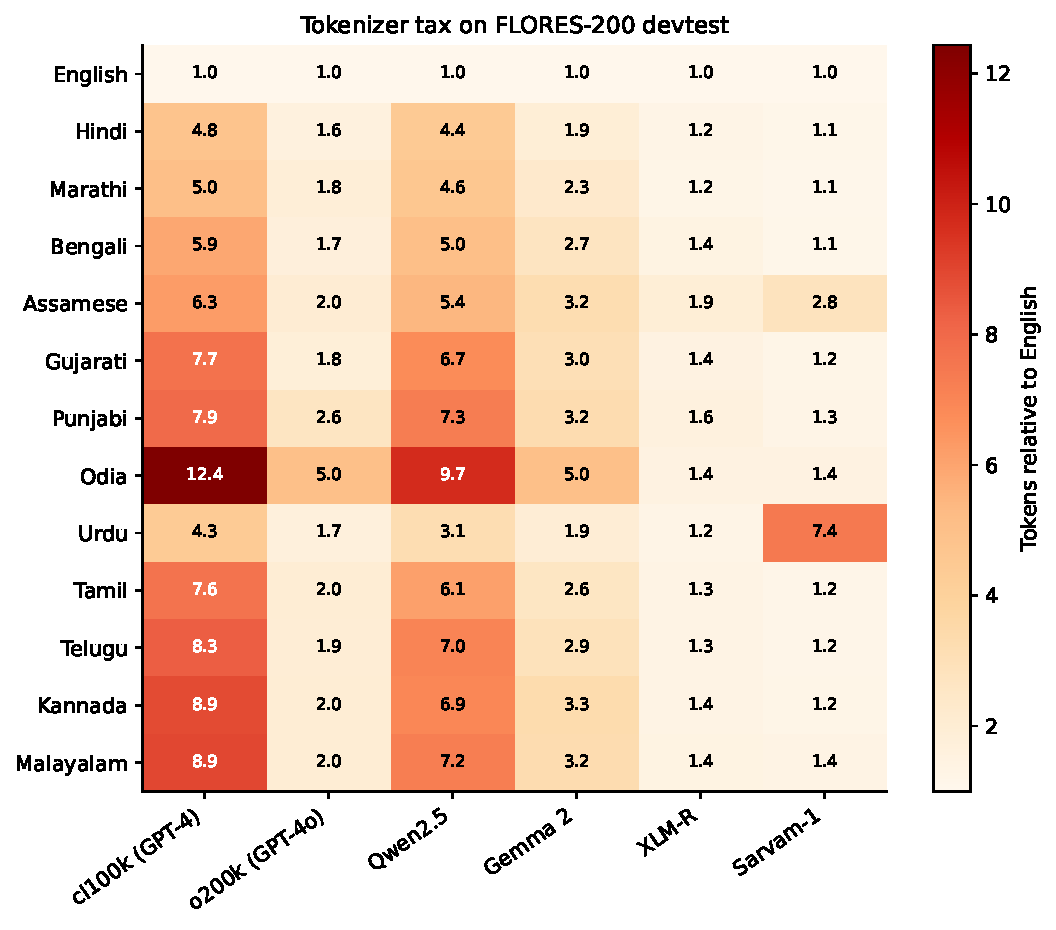
\includegraphics[width=\columnwidth]{fig_tax_heatmap}
  \caption{Tokenizer tax $T$ (tokens relative to English for the same FLORES-200 devtest content).}
  \label{fig:tax}
\end{figure}

\begin{figure}[t]
  \centering
  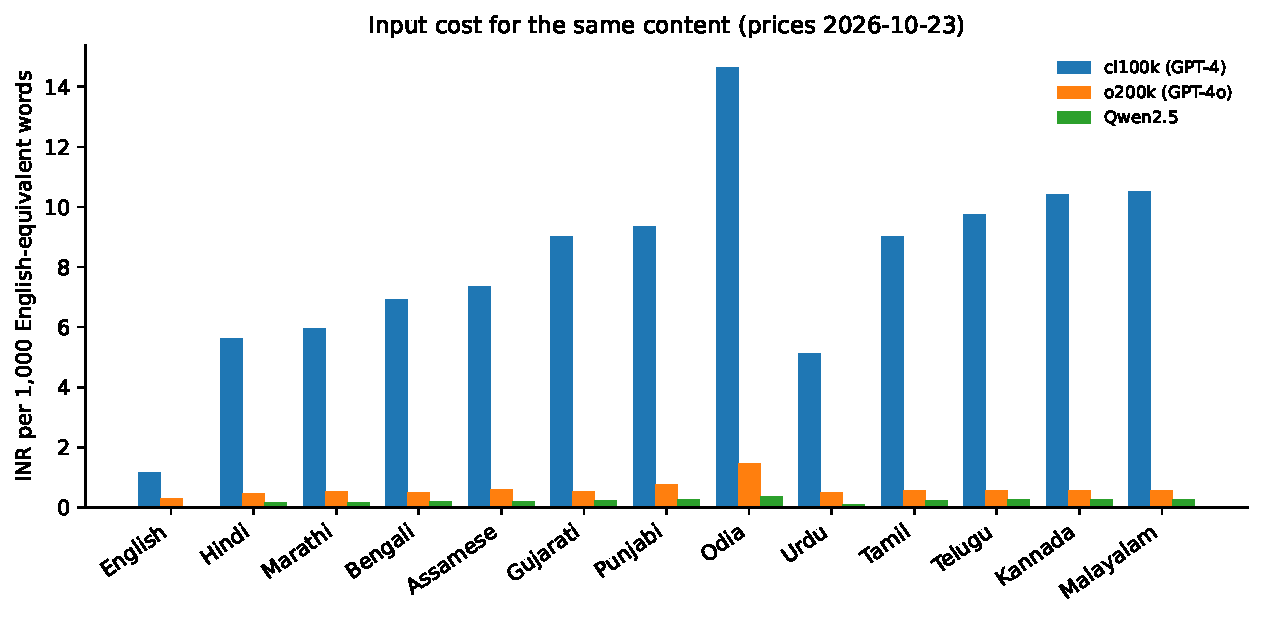
\includegraphics[width=\columnwidth]{fig_cost}
  \caption{Input cost in INR per 1{,}000 English-equivalent words at published API prices.}
  \label{fig:cost}
\end{figure}
